\documentclass{article}

% Langue
\usepackage[utf8]{inputenc}
\usepackage[T1]{fontenc}      
\usepackage[francais]{babel}

% Mise en forme générale
\usepackage[top=2.5cm,bottom=2.5cm,right=2.5cm,left=2.5cm]{geometry}

% Package divers
\usepackage{chemist} 
\usepackage[version=3]{mhchem}
\usepackage{chemfig}
\usepackage[squaren, Gray]{SIunits}
\usepackage{sistyle}
\usepackage[autolanguage]{numprint}
\usepackage{url}
\usepackage{rotating}
\usepackage{xcolor,colortbl}
\definecolor{Gray}{gray}{0.85}

\usepackage{hyperref}
\hypersetup{
    colorlinks,
    citecolor=black,
    filecolor=black,
    linkcolor=black,
    urlcolor=black
}

% Nouvelles commandes
\newcommand{\std}{\ensuremath{^{\circ}}}
\newcommand\ph{\ensuremath{\mathrm{pH}}}
\newcommand{\annexe}{\part{Annexes}\appendix}
\newcommand{\biblio}[1]{\bibliographystyle{plain}\bibliography{#1}\nocite{*}}

\newcommand{\doctitle}[1]{
	\title{#1}
	\author{\textbf{Groupe 124.3}\\
	\textsc{Frenyo} Péter (6266-12-00)\\
	\textsc{Gillain} Nathan (7879-12-00)\\
	\textsc{Lamine} Guillaume (7109-13-00)\\
	\textsc{Piraux} Pauline (2520-13-00)\\
	\textsc{Paris} Antoine (3158-13-00)\\
	\textsc{Quiriny} Simon (4235-13-00)\\
	\textsc{Schrurs} Sébastien (7978-13-00)}
	\date{\today}

	\begin{document}

	\maketitle
	\tableofcontents
}

\doctitle{Conception plus détaillée de la dernière étape du procédé :
la synthèse d'ammoniac proprement dite}

\section{Introduction}
Contrairement à ce que nous avons fait précedement nous allons nous intéressé
plus en détails à la dernière étape: la synthèse d'ammoniac proprement dite.
Dans un premier temps, nous étudierons les contraintes thermodynamiques de 
la réaction afin d'établir les conditions de cette réaction.
Dans un deuxième temps, nous simulerons le procédé à l'aide du logiciel
\textsc{Aspen+}.

\section{Etude thermodynamique}
\subsection{Etude qualitative des paramètres thermodynamiques }
\subsubsection{Pression}
Selon Le Chatelier: "Si une modification est imposée à un système chimique à 
l'état d'équilibre, il s'ensuit la réaction chimique qui s'oppose en partie
à la modification imposée; le système évolue vers un nouvel état d'équilibre"
\cite{LeChatelier}.

A température et volume constants, la pression d'un gaz dépend directement
du nombre de moles de gaz contenu dans une enceinte. On en déduit donc qu'une
augmentation de la pression favorise une diminution du nombre de moles.

Or notre procédé est régit par la réaction suivante :
\begin{chemmath} 
	N_2(g) + 3H_{2}O(g) \longrightarrow 2NH_3(g)
\end{chemmath} 

On observe que le nombre de moles de gaz produites est inférieur au nombre 
initial. Si nous voulons augmenter la quantité d'ammoniac produit, il faut 
une haute pression. 

Par ailleurs, une augmentation de la pression rapproche les molécules, ce qui
par conséquent augmente la possibilté que les molécules se heurtent aux 
catalyseurs, favorisant ainsi la réaction.

Cependant, les infrastructures à mettre en place pour supporter des pressions
importantes reviennent cheres ainsi que le procédé pour maintenir une haute pression.

En pratique, on procéde à un compromis entre la quantité produite et le coût des opérations.
La pression est de l'ordre de \unit{200}{\bbar} \cite{HaberB}.

\subsubsection{Température}
Notre réaction est exothermique, on observe que son $\Delta H$ est négatif.
Selon Le Chatelier, un diminution de température favorisera la réaction 
exothermique pour tempter de s'opposer à la diminution d'énergie \cite{LeChatelier}. 
Si nous voulons augmenter la quantité d'ammoniac produit, il faut une basse température.
Nous pouvons observer sur le graphique \ref{fig:constantK}, que 
la constante d'équilibre est élevée à basse température et faible à haute température.

\begin{figure}
	\centering
	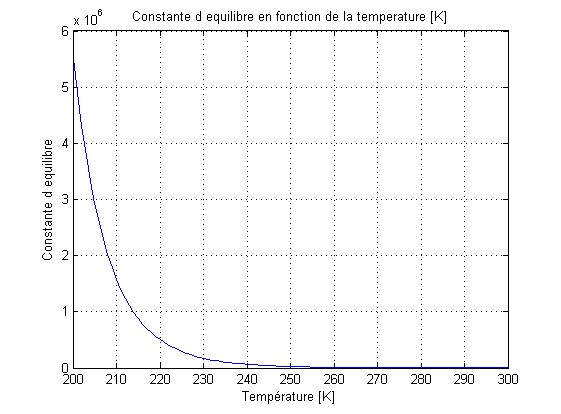
\includegraphics[scale=0.48]{media/grapheK200-300.jpg}
	\caption{Résultat du calcul de la constante d'équilibre.}
	\label{fig:constantK}
\end{figure}

Cependant, à basse température la réaction est ralentie. 

En pratique, on préfère produire une grande quantité d'ammoniac en un temps très court. 
La température avoisine les \unit{400-500}{\degreecelsius} \cite{HaberB}.

\subsection{Etude quantitative des paramètres thermodynamiques }
Nous avions d'abord fait l'hypothèse que la synthèse était complète.
Nous pouvons maintenant l'analyser plus en détails en la considérant
à l'équilibre thermodynamique. Nous ferons ici l'hypothèse du gaz
parfait, une étude plus rigoureuse à l'aide du logiciel \textsc{Aspen+}
sera faite par la suite. Notons à l'avance que nous travaillerons
à pression constante étant donné que nous sommes dans un système ouvert.
On se rend vite compte qu'une conversion complète n'est pas réalisable. 
Nous avons alors incorporé une boucle de recyclage des réactifs résiduels
afin de les renvoyer à l'entrée du réacteur. Cette boucle comprend une 
purge afin d'éviter l'accumulation d'argon présent dans l'air. 
% FIX : (et une surpression?)

Le tableau~\ref{tab:ammoniac} fait le bilan à l'équilibre thermodynamique.

\begin{table}[!ht]
	\begin{center}
		\begin{tabular}{c|ccc}
			Avancement & 
			\multicolumn{1}{c!{\makebox[0pt]{+}}}{\ce{1/2N2_{(g)}}} &
			\multicolumn{1}{c!{\makebox[0pt]{$\rightleftharpoons$}}}{\ce{3/2H2_{(g)}}} &
			\ce{NH3_{(g)}} \\
			\hline
			$n_i$ & $n_1$ & $n_2$ & $0$ \\
			$n_{eq}(x)$ & $n_1 - \frac{x}{2}$ & $n_2 - \frac{3x}{2}$ & $x$ \\
			\hline
			$a(x)$ & 
			%$\frac{2n_{1} - x}{2 n_{g,tot}} \frac{p_{tot}}{p \degree}$ 
			$\frac{2n_{1} - x}{2 n_{g,tot}} \frac{p_{tot}}{p_0}$ &
			$\frac{2n_{2} - 3x}{2 n_{g,tot}} \frac{p_{tot}}{p_0}$ &
			$\frac{x}{n_{g,tot}} \frac{p_{tot}}{p_0}$ \\
		\end{tabular}
		\caption{Tableau d'avancement de la réaction de synthèse de l'ammoniac.}
		\label{tab:ammoniac}
	\end{center}
\end{table}

Dans celui-ci, $n_1$, $n_2$ et $n_3$ sont respectivement les débits molaires 
d'azote, d'hydrogène et d'argon. La variable $x$ est l'avancement de la réaction. De plus,la somme des débits molaires de gaz
à l'équilibre est : $n_{g,tot} = n_1 + n_2 + n_3 - x$. 

On retire de cela et du tableau~\ref{tab:ammoniac}, une expression de la constante d'équilibre :

$$K(T) = \frac{4x\cdot p_0\cdot n_{g,tot}}{(2n_1 - x)^{1/2} (2n_2 - 3x)^{3/2} \cdot p_{tot}}.$$

Cette constante d'équilibre peut également être calculée en procédant de la même manière que pour le réformage primaire. 
% Comment citer une section en latex ??

Pour aider à visualiser l'analyse quantitative de la réaction, nous vous renvoyons à la figure~\ref{fig:purge1}.

\begin{figure}
	\centering
	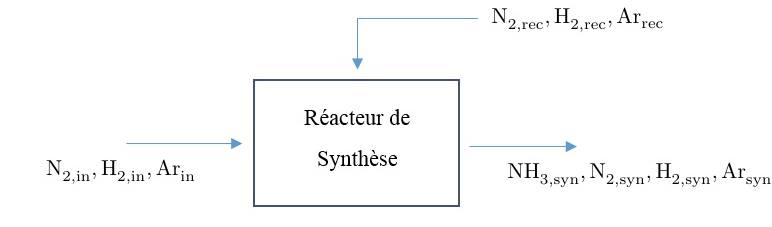
\includegraphics[scale=0.5]{media/reacteurNH3.jpg}
	\caption{Modélisation du recyclage des réactifs dans le réacteur de synthèse}
	\label{fig:purge1}
\end{figure}

En développant le problème dans le cas d'un recyclage avec purge, on a :

\begin{align}
	\notag
	\begin{cases}
	 n_1 = \ce{N2_{,in} + N2_{,rec}} \\
	 n_2 = \ce{H2_{,in} + H2_{,rec}} \\
	 n_3 = \ce{Ar_{in} + Ar_{rec}} \\
	\end{cases}
	 &  \text{et}  &
	\begin{cases}
	 \ce{N2_{,syn}} = n_1 - \frac{x}{2} \\
	 \ce{H2_{,syn}} = n_2 - \frac{3x}{2} \\
	 \ce{NH3_{,syn}} = x \\
	 \ce{Ar_{syn} = Ar_{in} + Ar_{rec}} \\ 
	\end{cases}
	\\
\end{align}

Les équations de gauche sont dues au recyclage et celles de droite 
à la conservation de la matière. Ensuite, nous avons les trois relations
de la purge où nous posons un coefficient $k$ de proportion entre ce qui
est recyclé et ce qui sort du réacteur de synthèse. On fait l'hypothèse
que la purge enlève une proportion égale de moles pour chaque composé.

$$
\begin{cases}
 k\cdot \ce{N2_{,syn}} = \ce{N2_{,rec}} \\ 
 k\cdot \ce{H2_{,syn}} = \ce{H2_{,rec}} & k \in [0 \text{(ouvert)}, 1 \text{(fermé)}[ \\
 k\cdot \ce{Ar_{syn}} = \ce{Ar_{rec}} \\
\end{cases}
$$

Enfin, il nous reste à imposer que en régime l'argon rentrant doit être égal
à l'argon purgé. C'est indispensable pour éviter une accumulation du composé
dans le réacteur, et une baisse du rendement. 
Il faut donc : $(1 - k)\ce{Ar_{syn}} = \ce{Ar_{in}}$.

A partir de ces différentes équations, nous pouvons exprimer l'ammoniac
sortant en fonction des composants à l'entrée, du coefficient, de la pression
totale et de la température. Les détails du calcul sont laissés à l'attention 
du lecteur. Nous arrivons finalement à l'équation~\eqref{eq:finale}, qui peut
être résolue numériquement à l'aide de l'outil \textsc{Matlab}.

\begin{align}
	K(T) & = \frac{4x\cdot p_0\cdot (\ce{N2_{,in} + H2_{,in} + Ar_{in}} - 
	\ce{NH3_{,syn}}(k + 1)) (1 - k)}{(\ce{2N2_{,in} - NH3_{,syn}})^{1/2} (\ce{2H2_{,in} - 3NH3_{,syn}})^{3/2} \cdot p_{tot}}
	\label{eq:finale}
\end{align}

Pour pouvoir complèter notre outil de gestion, nous exprimons les entrées 
en fonction du débit d'ammoniac voulue, de $k$, de la pression et de la
température. Pour cela nous nous plaçons dans le cas idéal stœchiométrique,
où aucuns des composants n'est en excès. De plus, nous prenons en compte la 
concentration d'argon naturellemnt dans l'air. 
 
$$
\begin{cases}
 \ce{N2_{,in}} = \ce{78Ar_{in}}\\ 
 \ce{N2_{,in}} = \ce{1/3H2_{,in}} \\
\end{cases}
$$
 
A l'aide de notre programme \textsc{Matlab} résolvant l'équation finale~\eqref{eq:finale}  nous avons tracer des graphiques mettant en valeur nos résultats.

\begin{figure}
	\centering
	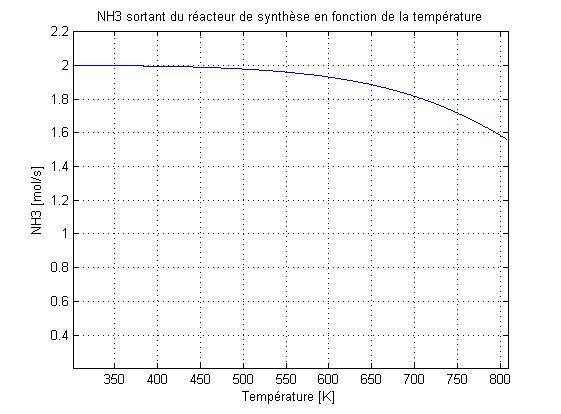
\includegraphics[scale=0.5]{media/purgeTemperature.jpg} 
	\caption{Modélisation de la production de \chemform{NH_3} du procédé \textsc{Haber Bosh}}
	\label{fig:purgeTemperature}
\end{figure}

Le graphe \ref{fig:purgeTemperature} a été réalisé à une pression constante de \unit{270}{\bbar}, pour \unit{1}{\mole\per\second} de \chemform{N_2}, une purge de 10\% et pour des températures de \unit{300-800}{\kelvin}. On observe conformément à nos attentes que le débit de \chemform{NH_3} diminue lorsque la température augmente. Le rendement est proche de 100\% à température ambiante, cela s'explique également par le recyclage des réactifs. A \unit{800}{\kelvin} le rendement chute à 80\%.

\begin{figure}
	\centering
	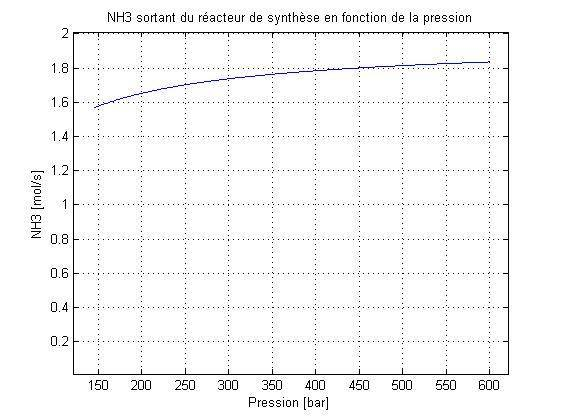
\includegraphics[scale=0.5]{media/purgePression.jpg} 
	\caption{Modélisation de la production de \chemform{NH_3} du procédé \textsc{Haber Bosh}}
	\label{fig:purgePression}
\end{figure}

Le graphe \ref{fig:purgePression} a été réalisé à une température constante de \unit{750}{\kelvin}, pour \unit{1}{\mole\per\second} de \chemform{N_2}, une purge de 10\% et pour des pressions de \unit{150-600}{\bbar}. On observe conformément à nos attentes que le débit de \chemform{NH_3} augmente lorsque la pression augmente aussi. A \unit{200}{bbar} le rendement est de l'ordre de 80\%, tandis que lorsque le pression est supérieure à \unit{450}{bbar} le rendement dépasse les 90\%.


\begin{figure}
	\centering
	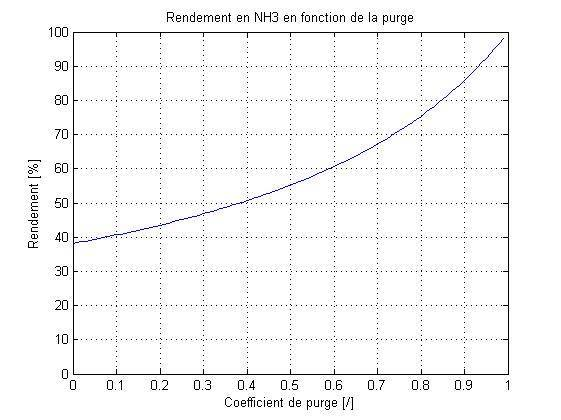
\includegraphics[scale=0.5]{media/purge.jpg} 
	\caption{Modélisation de la production de \chemform{NH_3} du procédé \textsc{Haber Bosh}}
	\label{fig:purge}
\end{figure}

Le graphe \ref{fig:purge} a été réalisé à une température constante de \unit{750}{\kelvin}, une pression constante de \unit{270}{\bbar}, pour \unit{1}{\mole\per\second} de \chemform{N_2} et pour des purges de 10\% à 100\%. On observe conformément à nos attentes que le débit de \chemform{NH_3} diminue lorsque la purge augmente. Lorsque la purge est totale le rendement est de 40\% tandis qu'avec une purge de 10\% nous atteignons 85\%.


\section{Utilisation du logiciel \textsc{Aspen+}}
Nous avons ensuite utilisée le logiciel \textsc{Aspen+}
afin de simuler la synthèse de l'ammoniac. Pour cela
nous avons construit le flow-sheet présenté à la figure
\ref{fig:flow-sheet-aspen}. 

\begin{figure}
	\centering
	\rotatebox{90}{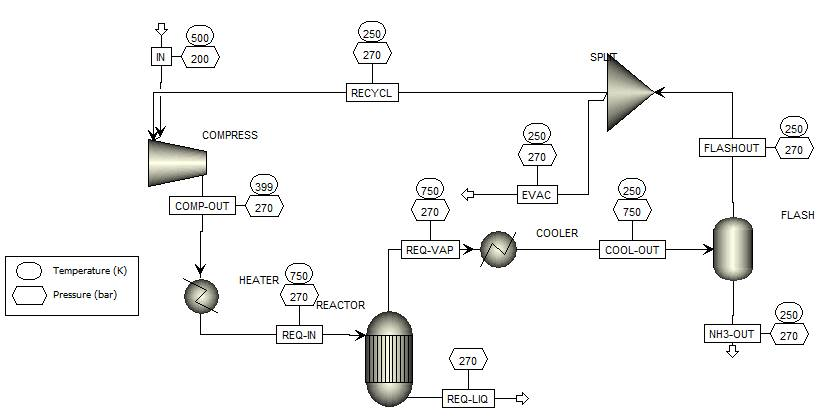
\includegraphics[scale=0.7]{media/flow-sheet.jpg}}
	\caption{Flow-sheet du procédé de synthèse de l'ammoniac
	réalisé avec \textsc{Aspen+}.}
	\label{fig:flow-sheet-aspen}
\end{figure}

Pour la simulation, nous avons utilisé la méthode
thermodynamique \textsc{SRK} qui est particulièrement
approprié pour les réactions entre gaz avec une pression
et une température élevée. Nous avons choisi d'utiliser
une purge de 4\%. La simulation nous fournit les résultats
présente à la figure \ref{fig:resultats-aspen}.

\begin{figure}
	\centering
	\rotatebox{90}{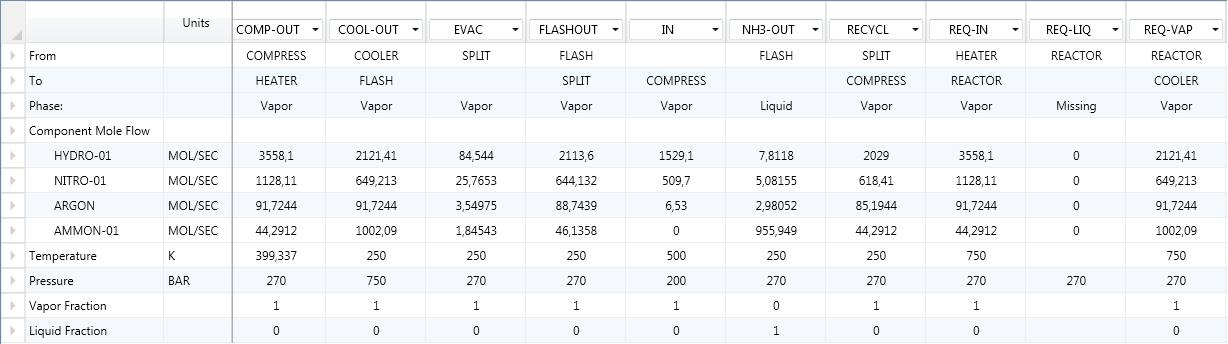
\includegraphics[scale=0.48]{media/results.jpg}}
	\caption{Résultats du procédé de synthèse de l'ammoniac
	réalisé avec \textsc{Aspen+}.}
	\label{fig:resultats-aspen}
\end{figure}

Ces résultats sont assez proches de ceux fournis par
l'outil de gestion. En effet, en prenant les valeurs
d'entrées nécessaires à la production à \unit{1000}{\kelvin} de
\unit{1500}{\ton\per\dday}, soit \unit{1019.40}{\mole\per\second},
de \chemform{NH_3} avec notre outil de gestion, notre simulation \textsc{Aspen+}
nous fournit un débit de \unit{955.949}{\mole\per\second} (ligne AMMON-01, colonne NH3-OUT),
soit un rendement de 93.77\%. Le débit de sortie de \chemform{NH_3}
est inférieur à celui obtenu avec notre outil de gestion étant donné que
ce dernier considère la réaction principale comme complète, tandis qu'\textsc{Aspen+}
rajoute la purge, nécessaire pour éviter l'accumulation d'\chemform{Ar}
mais ayant comme conséquence le défaussage d'une certaine quantité de
\chemform{N_2} et de \chemform{H_2}, et calcule également automatiquement un rendement
standard pour les réacteurs, séparateurs et tout composant de notre système
(nous pouvons d'ailleurs remarquer que la colonne NH3-OUT, indiquant le débit
de sortie supposé ne contenir que du \chemform{NH_3}, contient quand même du 
\chemform{N_2}, \chemform{H_2} et \chemform{Ar}, 
tout simplement parce qu'Aspen représente la réalité des choses et 
un séparateur n'est jamais parfait).

\biblio{sources-tache2}

\end{document}
